% !TEX TS-program = lualatex
% !TEX encoding = UTF-8 Unicode
% !TEX spellcheck = en_US
% © 2024 Moritz Brinkmann, CC-by-sa
% https://ma.latexkurs.de

\documentclass[
	vorläufig=false,
	datum=2023-03-09,
	titel={day two},
	web=true,handout,
	kursB,
	noshortverb,
	englisch=true,
]{../tex/latexkurs-slides}

%%%%%%%% Eval: %%%%%%%%
%%% 1. Termin: APAL6
%%% 2. Termin: UKFED
\def\evallosungA{APAL6}
\def\evallosungB{UKFED}
%%%%%%%%%%%%%%%%%%%%%%%

\setcounter{section}{6}
\setcounter{teil}{6}

\usepackage{mathtools, siunitx, ulem, cases}
\normalem

\usepackage{marvosym}


\usepackage{array, booktabs, caption, pifont, tabularray}

\UseTblrLibrary{amsmath, booktabs, siunitx}

\usepackage{pgfplots}

\pgfplotsset{
	compat=1.18,
	width=7cm,
	lua backend=true,
}

\usetikzlibrary{calc, intersections, through, trees, positioning}

\begin{filecontents*}{data.dat}
time	values	error
0.00E+00	6.66E+01	7.85E-01
1.00E-01	4.69E+01	8.39E-01
2.00E-01	4.61E+01	1.33E+00
3.00E-01	5.87E+01	7.20E-01
4.00E-01	3.95E+01	1.75E+00
5.00E-01	5.47E+01	7.41E-01
6.00E-01	5.82E+01	6.22E-01
7.00E-01	4.26E+01	2.01E+00
8.00E-01	4.74E+01	8.85E-01
9.00E-01	5.75E+01	1.38E+00
1.00E+00	4.23E+01	1.75E+00
1.10E+00	4.10E+01	4.96E-01
1.20E+00	5.20E+01	9.71E-01
1.30E+00	4.14E+01	6.39E-01
1.40E+00	5.74E+01	1.71E+00
1.50E+00	6.74E+01	1.73E+00
1.60E+00	3.67E+01	1.88E+00
1.70E+00	4.57E+01	2.04E+00
1.80E+00	5.53E+01	1.76E+00
1.90E+00	5.36E+01	1.01E+00
2.00E+00	3.67E+01	1.71E+00
2.10E+00	4.77E+01	1.44E+00
2.20E+00	2.07E+01	1.21E+00
2.30E+00	4.21E+01	1.61E+00
2.40E+00	4.90E+01	1.24E+00
2.50E+00	2.95E+01	4.23E-01
2.60E+00	4.34E+01	7.34E-01
2.70E+00	5.01E+01	1.42E+00
2.80E+00	5.67E+01	2.00E+00
2.90E+00	4.16E+01	1.25E+00
3.00E+00	6.37E+01	1.14E+00
3.10E+00	5.19E+01	7.79E-01
3.20E+00	6.52E+01	1.09E+00
3.30E+00	4.72E+01	8.79E-01
3.40E+00	5.12E+01	2.29E+00
3.50E+00	4.09E+01	1.70E+00
3.60E+00	4.37E+01	1.14E+00
3.70E+00	5.63E+01	6.61E-01
3.80E+00	4.46E+01	1.79E+00
3.90E+00	4.47E+01	1.21E+00
4.00E+00	4.84E+01	1.55E+00
4.10E+00	5.31E+01	1.25E+00
4.20E+00	4.73E+01	1.56E+00
4.30E+00	4.47E+01	8.65E-01
4.40E+00	5.69E+01	1.49E+00
4.50E+00	5.10E+01	1.16E+00
4.60E+00	4.61E+01	9.93E-01
4.70E+00	5.39E+01	1.27E+00
4.80E+00	5.66E+01	6.96E-01
4.90E+00	5.48E+01	1.28E+00
5.00E+00	6.04E+01	1.01E+00
5.10E+00	5.96E+01	6.92E-01
5.20E+00	4.86E+01	2.09E+00
5.30E+00	6.14E+01	3.53E+00
5.40E+00	4.09E+01	6.52E-01
5.50E+00	3.89E+01	9.98E-01
5.60E+00	5.00E+01	1.06E+00
5.70E+00	3.54E+01	4.91E-01
5.80E+00	5.30E+01	1.25E+00
5.90E+00	3.34E+01	1.57E+00
6.00E+00	4.61E+01	1.20E+00
6.10E+00	4.18E+01	1.96E+00
6.20E+00	5.91E+01	6.14E-01
6.30E+00	3.65E+01	4.75E-01
6.40E+00	4.36E+01	5.77E-01
6.50E+00	5.05E+01	2.57E+00
6.60E+00	5.72E+01	1.23E+00
6.70E+00	3.58E+01	2.03E+00
6.80E+00	4.99E+01	5.78E-01
6.90E+00	2.99E+01	1.31E+00
7.00E+00	5.19E+01	7.83E-01
7.10E+00	6.05E+01	1.35E+00
7.20E+00	5.34E+01	1.65E+00
7.30E+00	6.39E+01	1.14E+00
7.40E+00	3.87E+01	8.47E-01
7.50E+00	5.40E+01	1.37E+00
7.60E+00	2.81E+01	1.95E+00
7.70E+00	4.92E+01	1.38E+00
7.80E+00	5.91E+01	1.81E+00
7.90E+00	4.31E+01	7.86E-01
8.00E+00	5.29E+01	1.26E+00
8.10E+00	5.58E+01	1.22E+00
8.20E+00	4.53E+01	9.30E-01
8.30E+00	4.91E+01	1.17E+00
8.40E+00	3.61E+01	1.20E+00
8.50E+00	5.85E+01	1.28E+00
8.60E+00	5.56E+01	9.99E-01
8.70E+00	4.01E+01	1.52E+00
8.80E+00	5.43E+01	5.87E-01
8.90E+00	4.71E+01	2.04E+00
9.00E+00	6.66E+01	9.54E-01
9.10E+00	6.56E+01	8.88E-01
9.20E+00	4.63E+01	1.31E+00
9.30E+00	4.37E+01	6.35E-01
9.40E+00	3.41E+01	1.48E+00
9.50E+00	4.31E+01	1.69E+00
9.60E+00	5.13E+01	9.08E-01
9.70E+00	5.78E+01	6.10E-01
9.80E+00	4.35E+01	5.23E-01
9.90E+00	4.56E+01	2.18E+00
1.00E+01	3.93E+01	1.87E+00
1.01E+01	3.78E+01	1.04E+00
1.02E+01	5.35E+01	7.32E-01
1.03E+01	3.84E+01	5.04E-01
1.04E+01	3.86E+01	3.05E+00
1.05E+01	5.82E+01	6.16E-01
1.06E+01	5.76E+01	8.33E-01
1.07E+01	4.81E+01	4.92E-01
1.08E+01	4.80E+01	1.58E+00
1.09E+01	5.20E+01	1.09E+00
1.10E+01	5.62E+01	1.78E+00
1.11E+01	5.22E+01	7.71E-01
1.12E+01	6.96E+01	9.44E-01
1.13E+01	4.42E+01	3.20E+00
1.14E+01	5.85E+01	1.24E+00
1.15E+01	5.72E+01	8.41E-01
1.16E+01	4.46E+01	5.64E-01
1.17E+01	4.10E+01	4.68E-01
1.18E+01	4.83E+01	2.23E+00
1.19E+01	4.77E+01	1.56E+00
1.20E+01	4.03E+01	1.33E+00
1.21E+01	4.50E+01	2.55E+00
1.22E+01	5.07E+01	1.56E+00
1.23E+01	5.84E+01	8.86E-01
1.24E+01	6.17E+01	6.23E-01
1.25E+01	5.66E+01	2.86E+00
1.26E+01	4.94E+01	7.67E-01
1.27E+01	4.58E+01	1.72E+00
1.28E+01	3.01E+01	1.95E+00
1.29E+01	5.98E+01	9.92E-01
1.30E+01	3.92E+01	5.37E-01
1.31E+01	5.37E+01	1.58E+00
1.32E+01	6.17E+01	1.34E+00
1.33E+01	5.46E+01	1.57E+00
1.34E+01	5.49E+01	1.28E+00
1.35E+01	4.73E+01	6.21E-01
1.36E+01	4.93E+01	1.26E+00
1.37E+01	6.05E+01	2.27E+00
1.38E+01	5.57E+01	1.78E+00
1.39E+01	5.10E+01	2.28E+00
1.40E+01	4.52E+01	8.72E-01
1.41E+01	6.48E+01	9.98E-01
1.42E+01	4.24E+01	1.33E+00
1.43E+01	2.83E+01	9.89E-01
1.44E+01	3.63E+01	1.02E+00
1.45E+01	5.53E+01	1.06E+00
1.46E+01	5.46E+01	9.29E-01
1.47E+01	5.26E+01	1.64E+00
1.48E+01	5.29E+01	8.76E-01
1.49E+01	7.10E+01	9.16E-01
1.50E+01	5.68E+01	1.32E+00
1.51E+01	5.07E+01	1.52E+00
1.52E+01	2.40E+01	4.16E-01
1.53E+01	4.97E+01	1.12E+00
1.54E+01	4.50E+01	9.60E-01
1.55E+01	6.19E+01	1.60E+00
1.56E+01	6.02E+01	1.82E+00
1.57E+01	5.13E+01	1.06E+00
1.58E+01	4.44E+01	1.20E+00
1.59E+01	4.01E+01	6.17E-01
1.60E+01	3.64E+01	9.69E-01
1.61E+01	6.83E+01	2.52E+00
1.62E+01	4.72E+01	1.18E+00
1.63E+01	3.80E+01	1.33E+00
1.64E+01	5.17E+01	6.16E-01
1.65E+01	4.98E+01	9.33E-01
1.66E+01	5.02E+01	9.41E-01
1.67E+01	4.64E+01	8.34E-01
1.68E+01	5.47E+01	1.16E+00
1.69E+01	5.30E+01	1.91E+00
1.70E+01	7.31E+01	2.17E+00
1.71E+01	6.12E+01	1.02E+00
1.72E+01	3.09E+01	8.66E-01
1.73E+01	3.32E+01	6.54E-01
1.74E+01	2.03E+01	7.38E-01
1.75E+01	6.02E+01	1.47E+00
1.76E+01	3.72E+01	1.35E+00
1.77E+01	5.02E+01	1.04E+00
1.78E+01	5.91E+01	1.63E+00
1.79E+01	6.53E+01	7.36E-01
1.80E+01	4.99E+01	5.68E-01
1.81E+01	4.48E+01	7.96E-01
1.82E+01	3.85E+01	7.70E-01
1.83E+01	5.06E+01	5.57E-01
1.84E+01	5.26E+01	2.25E+00
1.85E+01	3.05E+01	5.72E-01
1.86E+01	5.20E+01	1.86E+00
1.87E+01	4.73E+01	7.05E-01
1.88E+01	3.70E+01	1.94E+00
1.89E+01	3.72E+01	8.31E-01
1.90E+01	4.68E+01	5.16E-01
1.91E+01	3.63E+01	5.35E-01
1.92E+01	5.29E+01	2.91E+00
1.93E+01	4.74E+01	7.59E-01
1.94E+01	6.16E+01	1.58E+00
1.95E+01	6.52E+01	1.08E+00
1.96E+01	6.26E+01	1.30E+00
1.97E+01	4.28E+01	1.37E+00
1.98E+01	5.49E+01	1.78E+00
1.99E+01	3.35E+01	6.29E-01
2.00E+01	3.44E+01	1.46E+00
2.01E+01	3.58E+01	9.79E-01
2.02E+01	6.22E+01	7.06E-01
2.03E+01	5.62E+01	4.09E+00
2.04E+01	6.07E+01	6.90E-01
2.05E+01	3.86E+01	6.46E-01
2.06E+01	5.57E+01	6.94E-01
2.07E+01	4.95E+01	9.53E-01
2.08E+01	3.80E+01	1.02E+00
2.09E+01	4.75E+01	7.88E-01
2.10E+01	5.03E+01	1.16E+00
2.11E+01	6.54E+01	1.47E+00
2.12E+01	1.93E+01	1.14E+00
2.13E+01	5.49E+01	7.27E-01
2.14E+01	4.86E+01	1.71E+00
2.15E+01	4.69E+01	1.72E+00
2.16E+01	5.22E+01	1.07E+00
2.17E+01	4.38E+01	1.57E+00
2.18E+01	5.01E+01	1.59E+00
2.19E+01	4.81E+01	1.14E+00
2.20E+01	5.21E+01	9.45E-01
2.21E+01	6.78E+01	1.33E+00
2.22E+01	6.24E+01	9.30E-01
2.23E+01	6.51E+01	7.59E-01
2.24E+01	6.74E+01	2.71E+00
2.25E+01	6.06E+01	1.45E+00
2.26E+01	6.12E+01	1.60E+00
2.27E+01	3.66E+01	7.60E-01
2.28E+01	4.53E+01	1.17E+00
2.29E+01	4.14E+01	1.27E+00
2.30E+01	4.64E+01	7.97E-01
2.31E+01	5.45E+01	5.74E-01
2.32E+01	6.32E+01	1.16E+00
2.33E+01	4.05E+01	7.92E-01
2.34E+01	4.66E+01	2.29E+00
2.35E+01	4.22E+01	1.17E+00
2.36E+01	5.09E+01	6.21E-01
2.37E+01	5.64E+01	6.97E-01
2.38E+01	3.90E+01	1.88E+00
2.39E+01	5.83E+01	2.15E+00
2.40E+01	5.34E+01	1.58E+00
2.41E+01	7.69E+01	1.41E+00
2.42E+01	4.52E+01	1.61E+00
2.43E+01	4.72E+01	1.49E+00
2.44E+01	3.63E+01	1.03E+00
2.45E+01	5.24E+01	1.10E+00
2.46E+01	6.34E+01	9.49E-01
2.47E+01	4.43E+01	9.20E-01
2.48E+01	6.60E+01	9.95E-01
2.49E+01	5.74E+01	1.24E+00
2.50E+01	4.18E+01	5.03E-01
2.51E+01	4.65E+01	2.06E+00
2.52E+01	6.10E+01	1.30E+00
2.53E+01	5.98E+01	1.29E+00
2.54E+01	4.79E+01	3.32E+00
2.55E+01	5.65E+01	5.72E-01
2.56E+01	4.07E+01	2.31E+00
2.57E+01	4.51E+01	9.00E-01
2.58E+01	5.86E+01	1.08E+00
2.59E+01	6.17E+01	1.34E+00
2.60E+01	2.70E+01	1.35E+00
2.61E+01	5.84E+01	1.87E+00
2.62E+01	3.46E+01	1.32E+00
2.63E+01	5.07E+01	6.47E-01
2.64E+01	3.40E+01	5.21E-01
2.65E+01	5.52E+01	6.66E-01
2.66E+01	3.79E+01	1.29E+00
2.67E+01	5.49E+01	1.30E+00
2.68E+01	5.71E+01	1.47E+00
2.69E+01	4.19E+01	6.68E-01
2.70E+01	3.63E+01	1.21E+00
2.71E+01	4.70E+01	1.41E+00
2.72E+01	5.15E+01	6.47E-01
2.73E+01	5.80E+01	1.02E+00
2.74E+01	5.65E+01	1.17E+00
2.75E+01	6.35E+01	1.02E+00
2.76E+01	6.31E+01	8.30E-01
2.77E+01	5.89E+01	1.97E+00
2.78E+01	5.79E+01	8.54E-01
2.79E+01	5.77E+01	1.38E+00
2.80E+01	5.05E+01	7.25E-01
2.81E+01	3.12E+01	1.46E+00
2.82E+01	5.40E+01	1.97E+00
2.83E+01	5.03E+01	7.23E-01
2.84E+01	4.98E+01	9.58E-01
2.85E+01	3.25E+01	1.29E+00
2.86E+01	6.23E+01	2.91E+00
2.87E+01	6.00E+01	3.00E+00
2.88E+01	3.88E+01	1.18E+00
2.89E+01	2.40E+01	3.06E-01
2.90E+01	4.14E+01	1.95E+00
2.91E+01	4.50E+01	1.88E+00
2.92E+01	5.46E+01	7.47E-01
2.93E+01	6.36E+01	3.16E+00
2.94E+01	4.79E+01	1.65E+00
2.95E+01	5.00E+01	1.02E+00
2.96E+01	4.89E+01	1.15E+00
2.97E+01	7.02E+01	1.13E+00
2.98E+01	5.06E+01	8.11E-01
2.99E+01	4.17E+01	1.12E+00
3.00E+01	5.95E+01	1.64E+00
3.01E+01	7.12E+01	2.67E+00
3.02E+01	5.60E+01	1.11E+00
3.03E+01	4.37E+01	2.29E+00
3.04E+01	5.86E+01	1.82E+00
3.05E+01	5.23E+01	8.67E-01
3.06E+01	2.68E+01	5.97E-01
3.07E+01	5.83E+01	2.14E+00
3.08E+01	6.14E+01	6.73E-01
3.09E+01	2.63E+01	1.09E+00
3.10E+01	2.87E+01	4.18E-01
3.11E+01	2.89E+01	2.33E+00
3.12E+01	4.29E+01	4.87E-01
3.13E+01	4.83E+01	6.91E-01
3.14E+01	4.86E+01	9.55E-01
3.15E+01	4.42E+01	3.41E+00
3.16E+01	3.86E+01	7.43E-01
3.17E+01	4.80E+01	9.79E-01
3.18E+01	5.86E+01	1.62E+00
3.19E+01	6.93E+01	2.05E+00
3.20E+01	4.94E+01	1.13E+00
3.21E+01	4.71E+01	1.38E+00
3.22E+01	4.33E+01	1.48E+00
3.23E+01	4.20E+01	5.80E-01
3.24E+01	6.51E+01	1.66E+00
3.25E+01	5.12E+01	1.70E+00
3.26E+01	3.86E+01	2.07E+00
3.27E+01	6.02E+01	1.08E+00
3.28E+01	4.41E+01	2.09E+00
3.29E+01	6.00E+01	6.15E-01
3.30E+01	3.13E+01	7.23E-01
3.31E+01	4.89E+01	1.22E+00
3.32E+01	4.50E+01	1.34E+00
3.33E+01	4.79E+01	2.36E+00
3.34E+01	4.55E+01	1.37E+00
3.35E+01	5.42E+01	1.39E+00
3.36E+01	4.30E+01	1.36E+00
3.37E+01	4.44E+01	1.88E+00
3.38E+01	7.43E+01	1.18E+00
3.39E+01	2.73E+01	1.54E+00
3.40E+01	7.30E+01	9.53E-01
3.41E+01	3.71E+01	9.57E-01
3.42E+01	5.23E+01	8.74E-01
3.43E+01	5.28E+01	1.61E+00
3.44E+01	5.47E+01	1.41E+00
3.45E+01	4.27E+01	1.53E+00
3.46E+01	6.49E+01	1.57E+00
3.47E+01	5.25E+01	1.19E+00
3.48E+01	4.13E+01	1.04E+00
3.49E+01	5.40E+01	2.43E+00
3.50E+01	3.93E+01	1.01E+00
3.51E+01	6.76E+01	2.05E+00
3.52E+01	4.95E+01	1.45E+00
3.53E+01	3.57E+01	1.15E+00
3.54E+01	3.71E+01	1.06E+00
3.55E+01	4.85E+01	7.94E-01
3.56E+01	4.93E+01	1.68E+00
3.57E+01	5.23E+01	1.18E+00
3.58E+01	5.00E+01	5.78E-01
3.59E+01	5.48E+01	1.02E+00
3.60E+01	5.37E+01	1.06E+00
3.61E+01	4.53E+01	2.55E+00
3.62E+01	5.46E+01	8.26E-01
3.63E+01	6.08E+01	1.07E+00
3.64E+01	3.99E+01	2.25E+00
3.65E+01	6.29E+01	1.55E+00
3.66E+01	4.53E+01	1.03E+00
3.67E+01	3.44E+01	1.70E+00
3.68E+01	3.71E+01	1.00E+00
3.69E+01	4.67E+01	1.24E+00
3.70E+01	4.78E+01	5.79E-01
3.71E+01	5.35E+01	1.07E+00
3.72E+01	3.83E+01	6.43E-01
3.73E+01	5.06E+01	1.06E+00
3.74E+01	4.68E+01	7.73E-01
3.75E+01	5.29E+01	9.46E-01
3.76E+01	5.57E+01	1.94E+00
3.77E+01	5.68E+01	8.31E-01
3.78E+01	4.42E+01	2.63E+00
3.79E+01	4.83E+01	1.94E+00
3.80E+01	3.86E+01	4.92E-01
3.81E+01	3.34E+01	2.24E+00
3.82E+01	4.75E+01	1.05E+00
3.83E+01	2.56E+01	1.31E+00
3.84E+01	5.18E+01	1.03E+00
3.85E+01	4.99E+01	8.12E-01
3.86E+01	4.70E+01	1.23E+00
3.87E+01	5.43E+01	7.25E-01
3.88E+01	4.48E+01	1.39E+00
3.89E+01	3.59E+01	4.71E-01
3.90E+01	5.57E+01	7.98E-01
3.91E+01	4.42E+01	1.44E+00
3.92E+01	4.87E+01	1.05E+00
3.93E+01	3.95E+01	9.74E-01
3.94E+01	5.41E+01	9.57E-01
3.95E+01	6.38E+01	1.40E+00
3.96E+01	6.93E+01	1.08E+00
3.97E+01	3.81E+01	1.71E+00
3.98E+01	5.75E+01	9.81E-01
3.99E+01	4.08E+01	8.44E-01
4.00E+01	4.33E+01	6.36E-01
4.01E+01	5.20E+01	2.65E+00
4.02E+01	4.45E+01	1.17E+00
4.03E+01	4.69E+01	5.40E-01
4.04E+01	5.04E+01	7.99E-01
4.05E+01	3.88E+01	1.56E+00
4.06E+01	3.82E+01	2.50E+00
4.07E+01	6.13E+01	1.03E+00
4.08E+01	5.37E+01	1.73E+00
4.09E+01	3.65E+01	7.05E-01
4.10E+01	5.58E+01	2.33E+00
4.11E+01	4.31E+01	1.68E+00
4.12E+01	4.71E+01	1.88E+00
4.13E+01	5.34E+01	6.56E-01
4.14E+01	5.81E+01	2.19E+00
4.15E+01	5.37E+01	2.04E+00
4.16E+01	4.60E+01	2.04E+00
4.17E+01	4.09E+01	6.37E-01
4.18E+01	5.57E+01	1.28E+00
4.19E+01	4.50E+01	1.82E+00
4.20E+01	5.15E+01	7.08E-01
4.21E+01	5.59E+01	1.48E+00
4.22E+01	5.77E+01	1.36E+00
4.23E+01	3.91E+01	7.41E-01
4.24E+01	6.75E+01	2.28E+00
4.25E+01	4.80E+01	8.55E-01
4.26E+01	3.67E+01	4.14E-01
4.27E+01	4.70E+01	1.90E+00
4.28E+01	6.39E+01	9.71E-01
4.29E+01	4.31E+01	1.02E+00
4.30E+01	4.46E+01	1.21E+00
4.31E+01	6.14E+01	1.05E+00
4.32E+01	3.56E+01	1.40E+00
4.33E+01	4.64E+01	2.18E+00
4.34E+01	4.33E+01	6.35E-01
4.35E+01	4.83E+01	1.71E+00
4.36E+01	5.28E+01	7.55E-01
4.37E+01	5.45E+01	1.02E+00
4.38E+01	3.91E+01	1.80E+00
4.39E+01	5.58E+01	7.13E-01
4.40E+01	4.18E+01	2.28E+00
4.41E+01	4.45E+01	7.46E-01
4.42E+01	5.18E+01	1.95E+00
4.43E+01	5.49E+01	6.38E-01
4.44E+01	3.89E+01	1.28E+00
4.45E+01	5.81E+01	2.80E+00
4.46E+01	4.57E+01	1.48E+00
4.47E+01	5.39E+01	1.10E+00
4.48E+01	4.04E+01	5.05E-01
4.49E+01	6.09E+01	1.02E+00
4.50E+01	4.89E+01	2.03E+00
4.51E+01	5.14E+01	1.64E+00
4.52E+01	4.41E+01	1.29E+00
4.53E+01	5.64E+01	2.14E+00
4.54E+01	5.29E+01	1.06E+00
4.55E+01	4.25E+01	1.52E+00
4.56E+01	6.14E+01	1.17E+00
4.57E+01	5.54E+01	4.42E+00
4.58E+01	6.05E+01	6.63E-01
4.59E+01	4.45E+01	1.39E+00
4.60E+01	4.96E+01	1.55E+00
4.61E+01	4.80E+01	1.72E+00
4.62E+01	4.71E+01	1.38E+00
4.63E+01	5.64E+01	1.33E+00
4.64E+01	6.41E+01	6.88E-01
4.65E+01	4.98E+01	6.06E-01
4.66E+01	4.38E+01	1.50E+00
4.67E+01	4.93E+01	8.41E-01
4.68E+01	5.32E+01	1.04E+00
4.69E+01	5.28E+01	8.75E-01
4.70E+01	5.99E+01	1.24E+00
4.71E+01	5.75E+01	1.13E+00
4.72E+01	5.94E+01	8.23E-01
4.73E+01	5.82E+01	1.56E+00
4.74E+01	5.81E+01	1.92E+00
4.75E+01	4.28E+01	1.45E+00
4.76E+01	5.74E+01	8.07E-01
4.77E+01	4.78E+01	1.04E+00
4.78E+01	6.29E+01	8.41E-01
4.79E+01	3.82E+01	1.51E+00
4.80E+01	4.88E+01	5.10E-01
4.81E+01	4.59E+01	7.59E-01
4.82E+01	4.29E+01	1.02E+00
4.83E+01	4.69E+01	5.59E-01
4.84E+01	3.71E+01	2.22E+00
4.85E+01	4.89E+01	9.84E-01
4.86E+01	6.28E+01	1.52E+00
4.87E+01	6.71E+01	8.16E-01
4.88E+01	5.40E+01	1.20E+00
4.89E+01	5.28E+01	5.46E-01
4.90E+01	4.49E+01	1.00E+00
4.91E+01	6.08E+01	3.44E+00
4.92E+01	3.97E+01	8.42E-01
4.93E+01	5.89E+01	8.16E-01
4.94E+01	4.69E+01	1.53E+00
4.95E+01	3.94E+01	9.02E-01
4.96E+01	3.80E+01	1.77E+00
4.97E+01	5.66E+01	2.26E+00
4.98E+01	3.88E+01	4.66E-01
4.99E+01	4.53E+01	8.86E-01
5.00E+01	5.09E+01	1.51E+00
\end{filecontents*}

%% Notes:
%% Zitate: Harvard-Methode (AuthorYear)


\begin{document}

\begin{frame}[t]{Contents}
	\tableofcontents
\end{frame}

%%%%%%%%%%%%%%%%%%%%%%%%%%%%%%%%%%%%%%%%%%%%%%%%%%%%%%%%%%%%%%%%%%%%%%%%%%%%%%%%%%%%%%%%%%%%%%%%%%%%%%%%%%
\teil{Bibliographies}
%%%%%%%%%%%%%%%%%%%%%%%%%%%%%%%%%%%%%%%%%%%%%%%%%%%%%%%%%%%%%%%%%%%%%%%%%%%%%%%%%%%%%%%%%%%%%%%%%%%%%%%%%%

\begin{frame}[fragile]{Bibliography}
\begin{itemize}
	\item Bibliography contains a list of used sources and possibly further literature.
	\item Different citation styles depending on the field of study.
	\item (Rough) appearance of the bibliography is determined by the document class.
	\pause
	\item Two methods for creating the bibliography:
	\begin{enumerate}
		\item Manual method with the \verb|thebibliography| environment.
		\item Automatic method with \hologo{BibTeX}/\hologo{biber}.
	\end{enumerate}
\end{itemize}
\end{frame}


\begin{frame}[fragile,t]{Manual Method}
 Specific syntax for setting the bibliography:
	\begin{itemize}
		\item Environment \verb|\begin{thebibliography}{|\meta{Number}\verb|}|
		\item Listing of works using \verb|\bibitem{|\meta{Key}\verb|}| \meta{Text}
		\item Citing a work with \verb|\cite{|\meta{Key(s)}\verb|}| or \verb|\cite[|\meta{Page}\verb|]{|\meta{Key}\verb|}|
	\end{itemize}
	\vfill
\begin{lstlisting}
\begin{thebibliography}{9}
  \bibitem{frankfurt05} Harry G. Frankfurt:
    \textit{On Bullshit}, Princeton University Press,
    Princeton, New Jersey, 2005.
\end{thebibliography}
\end{lstlisting}
\vfill
\pause
\begin{itemize}
	\item Manual creation (and sorting) of the bibliography is very cumbersome.
	\item Entries not easily reusable.
	\pause
	\item[⇒] Program \verb|biber| takes over sorting and management of entries.
\end{itemize}
\end{frame}

\subsection{biblatex/biber}
\begin{frame}[fragile]{\BibTeX/\hologo{biber} Idea}
	\begin{itemize}
		\item Entries exist as text files (\verb|.bib|) in a predefined syntax.
		\item Reference in the document with \verb|\cite{mittelbach2004}|\pdfmarginpar{If you want non-cited references to appear in the bibliography, you can add them with \texttt{nocite\{\}}. \texttt{nocite{*}} inserts all items in the .bib file.}
		\item Program \verb|biber| automatically adds referenced source to bibliography.
		\item Appearance of the reference and bibliography entries can be configured in various ways.
		\item Access to a large number of available references.
	\end{itemize}
\end{frame}


\begin{frame}[b,fragile]{The \texttt{.bib} File}
Different bib items for different document types:
\begin{columns}
\begin{column}{.3\textwidth}
	\begin{itemize}
		\item \verb|@article|
		\item \verb|@book|
		\item \verb|@mvbook|
		\item \verb|@inbook|
		\item \verb|@suppbook|
	\end{itemize}
\end{column}
\begin{column}{.3\textwidth}
	\begin{itemize}
		\item \verb|@collection|
		\item \verb|@manual|
		\item \verb|@online|
		\item \verb|@patent|
		\item \verb|@periodical|
	\end{itemize}
\end{column}
\begin{column}{.4\textwidth}
	\begin{itemize}
		\item \verb|@proceedings|
		\item \verb|@thesis|
		\item \verb|@unpublished|
		\item …
		\item[]
\end{itemize}
\end{column}
\end{columns}
\vfill
Each item has various mandatory and optional fields.
\vfill
\begin{block}{Syntax of an Entry}
\verb|@|\meta{Item-Type}\verb|{|\meta{Ref-Key}\verb|,|\\
\verb|    |\meta{Field}\verb|    = {|\meta{Value}\verb|},|\\
\verb|    |\meta{Field}\verb|    = {|\meta{Value}\verb|},|\\
\verb|}|
\end{block}
\end{frame}

\begin{frame}[b,fragile]{The \texttt{.bib} File}
	\begin{itemize}
		\item Usage is unintuitive.
		\item Graphical interfaces make life easier.
		\\ e.\,g., \href{https://www.jabref.org/}{JabRef}, \href{https://www.bibsonomy.org/}{BibSonomy}, \href{https://www.citavi.com/de}{Citavi}, \href{https://endnote.com/}{EndNote}, \href{https://www.mendeley.com}{Mendeley}, \href{https://www.zotero.org}{Zotero}, …
		\item Direct online search e.\,g., at \href{http://primo.bib.uni-mannheim.de/}{UB} or \href{https://scholar.google.de}{Google Scholar}
	\end{itemize}
	\vfill
\begin{block}{Syntax of an Entry}
\verb|@|\meta{Item-Type}\verb|{|\meta{Ref-Key}\verb|,|\\
\verb|    |\meta{Field}\verb|    = {|\meta{Value}\verb|},|\\
\verb|    |\meta{Field}\verb|    = {|\meta{Value}\verb|},|\\
\verb|}|
\end{block}
\end{frame}



\begin{frame}[fragile]{Creating the Bibliography}
\begin{olcol}
\begin{block}{in the document}\vspace{-1ex}
\begin{lstlisting}[frame=none]
\usepackage[style=authoryear]{biblatex}
\addbibresource{bibfile.bib}
\begin{document}
  Text  ... \parencite{Tolkien54} ... text.
  \printbibliography
\end{document}
\end{lstlisting}
\vspace{-1ex}
\end{block}
\begin{block}{in the .bib file}\vspace{-1ex}
\begin{lstlisting}[frame=none]
@book{Tolkien54,
  author    ={Tolkien, John R. R.},
  title     ={The Lord of the Rings},
  publisher ={Allen \& Unwin},
  place     ={London},
  year      ={1954},
}
\end{lstlisting}
\vspace{-1ex}
\end{block}
%\begin{block}{on the Terminal}
%\promt \verb|lualatex document.tex|\\
%\promt \verb|biber document.bcf|\\
%\promt \verb|lualatex document.tex|
%\end{block}
\end{olcol}
\overleaf{tex11}
\end{frame}

\begin{frame}[fragile]{Citation and Bibliography Styles}
\begin{itemize}
\item \pkg{biblatex} supports many predefined styles:
\item \verb|\usepackage[style=|\meta{Style}\verb|]{biblatex}|
\end{itemize}
\begin{description}
\item[\texttt{numeric}] Standard style \hfill [1, 2, 4, 3, 7]
\item[\texttt{numeric-comp}] Compact version of \texttt{numeric} \hfill [1-4, 7]
\item[\texttt{alphabetic}] Abbreviations of author and year \hfill [Jon95] [JW86] 
\item[\texttt{authoryear}] Author-year style \hfill Jones 1995 
\item[\texttt{authoryear-ibid}] Multiple citations on one page are abbreviated with \emph{ibid.}
\end{description}
\begin{itemize}
\item Bibliography style is adapted to the citation style.
\item Can be changed with \verb|citestyle=| and \verb|bibstyle=|.
\end{itemize}
\overleaf{tex11}
\end{frame}

\begin{frame}{Citing}
\texttt{\textbackslash textcite\{\meta{key}\}} generates reference in the text: \hfill {\small van Mises (1962)}\\
\texttt{\textbackslash Textcite\{\meta{key}\}} generates reference at the beginning of the sentence: \hfill {\small Van Mises (1962)}\\
\texttt{\textbackslash parencite\{\meta{key}\}} generates reference in parentheses: \hfill {\small (van Mises 1962)}\\
\vfill

Optional arguments:\\
\texttt{\textbackslash parencite[\meta{Text before}][\meta{Text after}]\{\meta{key}\}}\\
\texttt{\textbackslash parencite[\meta{Text after}]\{\meta{key}\}}
\vfill\pause
%\begin{olcol}
\begin{arbeitsauftrag}
Create a \texttt{.bib} file with some entries and try to reference them in a document.

Generate your document and bibliography by calling \LuaLaTeX, \hologo{biber}, and \LuaLaTeX.
\end{arbeitsauftrag}
%\end{olcol}
%\overleaf{tex11}
\end{frame}


%%%%%%%%%%%%%%%%%%%%%%%%%%%%%%%%%%%%%%%%%%%%%%%%%%%%%%%%%%%%%%%%%%%%%%%%%%%%%%%%%%%%%%%%%%%%%%%%%%%%%%%%%%
\teil{Typesetting Mathematics}
%%%%%%%%%%%%%%%%%%%%%%%%%%%%%%%%%%%%%%%%%%%%%%%%%%%%%%%%%%%%%%%%%%%%%%%%%%%%%%%%%%%%%%%%%%%%%%%%%%%%%%%%%%

\subsection{Inline and Display Mode}
\begin{frame}[t]{Inline and Display Mode}
\begin{columns}
\begin{column}{.48\textwidth}
\begin{block}{Inline Mode}
\begin{itemize}
	\item Formulas appearing directly in the text flow
	\item Short formulas, mentioning variables
	\item Elements do not exceed the line height
	\item Limits are set \emph{beside} integrals, sums, and products
\end{itemize}
\end{block}

\end{column}
\begin{column}{.48\textwidth}
\begin{block}{Display Mode}
	\begin{itemize}
		\item Emphasizes important formulas
		\item Represents long calculations
		\item Complex formulas
		\item Multiply indexed quantities
		\item Nested fractions
		\item …
	\end{itemize}
\end{block}
\end{column}
\end{columns}
\end{frame}

\begin{frame}{Inline and Display Mode}
\rmfamily
\textbf{Inline Math:} $E=mc^2$ is known by every child, but hardly anyone can make more sense of it than with $\int^\infty_{-\infty}\sum_{n = 1}^5 dx$, where this formula simply makes no sense, but shows how limits look in \TeX\ typesetting.
\textbf{Inline Math with Displaystyle:} $E=mc^2$ is known by every child, but hardly anyone can make more sense of it than with $\displaystyle \int^\infty_{-\infty}\sum_{n = 1}^5 dx$, where this formula simply makes no sense, but shows how limits look in \TeX\ typesetting.
\textbf{Display Math:} $E=mc^2$ is known by every child, but hardly anyone can make more sense of it than with \[\int^\infty_{-\infty}\sum_{n = 1}^5 dx,\] where this second formula simply makes no sense, but shows how limits look in \TeX\ typesetting.
\end{frame}


\begin{frame}[t,fragile]{Inline and Display Mode}
\vspace*{-1em}

\begin{columns}[t]
\begin{column}{.48\textwidth}
\begin{block}{Inline Mode}
\verb|$|\meta{Formula}\verb|$|
\end{block}\vspace*{2.72em}

\begin{LTXexample}[pos=b]
The function $K(x)$ models $K$ depending on $x$.
\end{LTXexample}
\end{column}
\begin{column}{.48\textwidth}
\begin{block}{Display Mode}
\verb|\begin{equation}|\\
~~\meta{Formula}\\
\verb|\end{equation}|
\end{block}\vspace*{0.1ex}

\begin{LTXexample}[pos=b]
\begin{equation}
  K(x) = c \cdot x^{-a}
\end{equation}
\end{LTXexample}
\end{column}
\end{columns}
\end{frame}


\begin{frame}[fragile]{Multi-line Formulas}
	A series of equations aligned and arranged with respect to each other, for example used for:
	\begin{itemize}
		\item Derivations
		\item Summaries
		\item Comparison of formulas
	\end{itemize}
%	\pause
%	\sout{\TeX\ standard environment: \texttt{eqnarray}} \pause \alert{ugly}\\	\alert{better:}
	 \verb|align| environment from the \pkg{amsmath} package.
	\pause
\begin{LTXexample}
\begin{align}
a &= b, &
c &= d,\\
abc &= d \\
&= r
\end{align}
\end{LTXexample}
	without numbering: \verb|{align*}|
\end{frame}


\subsection{Basic Commands}
\begin{frame}[fragile]{Variables and Numbers}
	\begin{itemize}
		\item Variables are set in italics: \verb|$a$|: $a$
		\item Font depends on the document class!\\%
		(Grotesque, Serifs, etc.)
		\item Digits are automatically set correctly: $12.2$ instead of 12.2
	\end{itemize}
	\vfill
	Package \pkg{siunitx} allows typesetting of quantities and units
\begin{LTXexample}[pos=r]
\num{3.14159+-0.00001} \\
\SI{95}{\kilo\joule} \\
\si{\milli\meter}
\end{LTXexample}
(works in math mode and text mode)
\end{frame}

\begin{frame}[fragile]{Superscripts and Subscripts}
	\begin{itemize}
		\item Characters with special meaning: \verb|^| and \verb|_|
		\item Superscript: \verb|a^b|\hfill $a^b$
		\item Subscript: \verb|a_b|\hfill $a_b$
		\item Grouping is possible: \verb|a^{bc}|, \verb|a_{bc}|\hfill $a_{bc}$
		\item Combination is possible: \verb|a_b^c|\hfill $a_b^c$
		\item Without preceding character: \verb|^{235}U|\hfill $^{235}\mathrm U$
		\item Nesting only with grouping:\\%
		\verb|a_{b_{c_{d_{e_{f^g}}}}}^{h^{i^{j_k}}}| \hfill \Large $a_{b_{c_{d_{e_{f^g}}}}}^{h^{i^{j_k}}}$\normalsize
		\item[] \verb|a_b_c| produces an error!
	\end{itemize}
\end{frame}

\begin{frame}[fragile]{Operators}
Operator names are set upright and are predefined
	\begin{itemize}
		\item Correct: $\sin(x)$\quad Incorrect: $sin(x)$
	\end{itemize}
\begin{LTXexample}[pos=b]
$\sin(x) \cos(y) \tan(2\pi) \lim \arctan$
\end{LTXexample}
	\pause
	\begin{itemize}
		\item Package \pkg{amsopn} provides many definitions:
	\end{itemize}
\begin{lstlisting}
\arccos \arcsin \arg \cos \cot \coth \deg \det
\exp \gcd \inf \injlim \lg \lim \limsup \ln
\max \min \projlim \sec \sinh \sup \tanh
\end{lstlisting}
\end{frame}

\begin{frame}[fragile]{Brackets}
Bracketing large expressions can be problematic:
\begin{LTXexample}
\[ (
  \frac{\int^a x dx}{\sum_{n=1} x}
) \]
\end{LTXexample}
Better:
\begin{LTXexample}
\[ \left(
  \frac{\int^a x dx}{\sum_{n=1} x}
\right) \]
\end{LTXexample}
\end{frame}


\begin{frame}[fragile]{Brackets}
\begin{itemize}
\item \verb|\left| and \verb|\right| before everything that stretches
\item \verb|\left( \right]| also works
\item \verb|\left. \right)| provides adapted right bracket
\item Superscripts and subscripts are adjusted:
\end{itemize}
\begin{LTXexample}[pos=b]
\begin{displaymath}
  \left. \int_a^b f(x) \mathrm dx \right\vert_a^b
  \qquad
  \left\{ \int_a^b f(x) \mathrm dx \right]
\end{displaymath}
\end{LTXexample}
\end{frame}

\begin{frame}[fragile]{Limits}
\begin{itemize}
\item Specify limits using \verb|\limits|
\item Multi-line limits with \verb|\atop|
\end{itemize}
\begin{LTXexample}
\[
  \int_a^b
  \int\limits_a^b
  \sum_{n=1}^\infty
  \prod_{n = 1 \atop m = 2}
\]
\end{LTXexample}
\end{frame}

\begin{frame}[fragile]{Special Characters}
\begin{itemize}
\item Many characters are accessible by their names,
\item as well as Greek uppercase and lowercase letters
\end{itemize}
\begin{LTXexample}[preset=\vspace{-1em}]
\begin{align*}
  \nabla \square \\ 
  \partial \infty \\
  \pm \mp \\
  \alpha \beta \gamma \\
  \rho \varrho \\
  \kappa \varkappa \\
  \epsilon \varepsilon \\
  \theta \vartheta \\
   A B \Gamma 
\end{align*}
\end{LTXexample}
\pause
If you are looking for a symbol:\\
\texttt{texdoc \href{https://texdoc.org/serve/maths-symbols/0}{maths-symbols} \href{https://texdoc.org/serve/symbols-a4/0}{symbols-a4}}
or \alert{\href{http://detexify.kirelabs.org/classify.html}{Detexify}}
\end{frame}

\begin{frame}[fragile]{Roots}
\begin{LTXexample}[preset=\Large]
\[
  \sqrt{a_{n_{m_p}}}
  \quad
  \sqrt[3]{a}
\]
\end{LTXexample}
\pause
\begin{itemize}
\item Roots with deep descenders are unsightly \item[⇒] \verb|\smash[|\meta{t, b}\verb|]{|\meta{Formula}\verb|}|
\end{itemize}
\begin{LTXexample}[preset=\Large]
\[
  \sqrt{a_{n_{m_p}}}
  \quad
  \sqrt{
    \smash[b]{
      a_{n_{m_p}}
    }
  }
\]
\end{LTXexample}
\end{frame}


\begin{frame}[fragile]{Matrices}
\begin{LTXexample}
\[
  \begin{matrix}
    a_{11} & a_{12}\\
    a_{21} & a_{22}
  \end{matrix}
\]
\end{LTXexample}
\pause
\begin{LTXexample}
\[
  \left(
    \begin{matrix}
      a_{11} & a_{12}\\
      a_{21} & a_{22}
    \end{matrix}
  \right)
\]
\end{LTXexample}
\end{frame}


\begin{frame}[fragile]{Matrices}
Package \pkg{amsmath} defines additional matrix environments:\\[2em]
\begin{minipage}{3cm}
\[\begin{pmatrix}
a & b \\ c & d
\end{pmatrix}\]
\centering pmatrix
\end{minipage}
\begin{minipage}{3cm}
\[\begin{Vmatrix}
a & b \\ c & d
\end{Vmatrix}\]
\centering Vmatrix
\end{minipage}
\begin{minipage}{3cm}
\[\begin{vmatrix}
a & b \\ c & d
\end{vmatrix}\]
\centering vmatrix
\end{minipage}
\\[2em]
\begin{minipage}{3cm}
\[\begin{Bmatrix}
a & b \\ c & d
\end{Bmatrix}\]
\centering Bmatrix
\end{minipage}
\begin{minipage}{3cm}
\[\begin{bmatrix}
a & b \\ c & d
\end{bmatrix}\]
\centering bmatrix
\end{minipage}
\begin{minipage}{3cm}
\[\begin{smallmatrix}
a & b \\ c & d
\end{smallmatrix}\]\\
\centering smallmatrix
\end{minipage}
\end{frame}

\subsection{Numbering}
\begin{frame}[fragile]{Numbering of Cases}
Package \pkg{cases} provides numbering of case constructs:
\begin{LTXexample}[pos=b]
\begin{numcases}{E = mc^2}
  m \neq 0 & massless particles\\
  m < 0 & antiparticles (?)\\
  m > 0 & normal particles
\end{numcases}
\end{LTXexample}
\end{frame}

\begin{frame}{Application}
\begin{arbeitsauftrag}
Try to recreate the following example.
\end{arbeitsauftrag}
\rmfamily\vfill
The Maxwell equations represent the relationship between the electric field $\vec E$ and the magnetic field $\vec B$:
\begin{align*}
\vec \nabla \cdot \vec E &= \frac{\rho}{\varepsilon_0} & \vec \nabla \times \vec E &= - \frac{\partial \vec B}{\partial t}\\
\vec \nabla \cdot \vec B &= 0 & \vec \nabla \times \vec B &= \mu_0\varepsilon_0\frac{\partial \vec E}{\partial t}
\end{align*}
Formula \ref{eq:summe} adds all $a_i$ weighted by $c_i$.
\begin{align}
\sum_{i=1}^n c_i \cdot a_i  \label{eq:summe}
\end{align}
\end{frame}


%%%%%%%%%%%%%%%%%%%%%%%%%%%%%%%%%%%%%%%%%%%%%%%%%%%%%%%%%%%%%%%%%%%%%%%%%%%%%%%%%%%%%%%%%%%%%%%%%%%%%
\teil{Tables}
%%%%%%%%%%%%%%%%%%%%%%%%%%%%%%%%%%%%%%%%%%%%%%%%%%%%%%%%%%%%%%%%%%%%%%%%%%%%%%%%%%%%%%%%%%%%%%%%%%%%%

\begin{frame}[fragile]{Table Environment: tabular}
\texttt{\textbackslash begin\{tabular\}\{\meta{Column Specification}\}}
\vfill
\begin{olcol}
\begin{LTXexample}[pos=b]
\begin{tabular}{llr}
first & second & third entry \\
new line & & with two entries \\
third & line
\end{tabular}
\end{LTXexample}
\end{olcol}
\overleaf{tex13}
\end{frame}

\begin{frame}[fragile]{Column Types}
\begin{description}
\item[\texttt{l}] left-aligned column
\item[\texttt{c}] centered column
\item[\texttt{r}] right-aligned column
\item[\texttt{|}] vertical line between columns
\item[\texttt{||}] double line between columns %(not crossed out)
\item[\texttt{p{\meta{Width}}}] column with fixed width
%\item[\texttt{@{\meta{Content}}}] instead of column separation, set \verb/Content/
\item[\texttt{\kern-.95ex*{n}{\meta{short}}}] repeat \meta{short} $n$ times, e.\,g., \verb/*{3}{p{4cm}|}/
\end{description}
\end{frame}

\begin{frame}[fragile]{tabular}
\begin{LTXexample}[pos=b,preset={\small}]
\begin{tabular}{l|c||r|p{2cm}|c|}
left & center & right & four & five\\\hline\hline
left & center & & a exceptionally long fourth column that breaks\\\hline
& & & &
\end{tabular}
\end{LTXexample}
\end{frame}

\subsection[tabularray]{Different Column Widths}
%\nocite{tabularray}

\begin{frame}[fragile]{Different Column Widths}
\begin{itemize}
\item Package \pkg{tabularray} offers various design options for tables.
\item classic usage: \
\verb|\begin{tblr}{|\meta{column definitions}\verb|}|
\verb|\end{tblr}|
\item extended input options:\\
\verb|\begin{tblr}{colspec={|\meta{column definitions}\verb|}, |\meta{additional options}\verb|}|\\
~~~~\meta{table content}\\
\verb|\end{tblr}|
\end{itemize}
\end{frame}


\begin{frame}[fragile]{Table with \pkg{tabularray}}
\begin{LTXexample}[pos=b,preset={\small}]
\begin{tblr}{
    columns = {wd=2cm, halign=c},
    row{2-3} = {font=\itshape},
    vlines, hlines,
  }
  Alpha   & Beta  & Gamma  & Delta \\
  Epsilon & Zeta  & Eta    & Theta \\
  Iota    & Kappa & Lambda & Mu    \\
\end{tblr}
\end{LTXexample}
\end{frame}





\begin{frame}[fragile]{Different Column Widths}
New column type:
\begin{description}
\item[\texttt{X[\meta{Factor},\meta{Type}]}] (left-aligned) column with variable width
\end{description}
\vfill

Available width is evenly distributed among all \verb|X|-columns:

\begin{LTXexample}[width=.4\textwidth]
\begin{tblr}{|l|l|r|}
 a a & b b & c c
\end{tblr}
\end{LTXexample}
\begin{LTXexample}[width=.4\textwidth]
\begin{tblr}{|l|X|r|}
 a a & b b & c c
\end{tblr}
\end{LTXexample}
\begin{LTXexample}[width=.4\textwidth]
\begin{tblr}{|X[1]|X[2]|X[3]|}
 a a & b b & c c
\end{tblr}
\end{LTXexample}
\end{frame}


\begin{frame}[fragile]{Line Breaks in Cells}
Rows can be broken with \verb|{ \\ }| if the cell content is enclosed:

\begin{LTXexample}[width=.4\textwidth]
\begin{tblr}{|X[r]|X[2,c]|X|}
 a a & {b b\\b b} & c c
\end{tblr}
\end{LTXexample}
\end{frame}


\begin{frame}[fragile]{Vertical Alignment}
Row types \texttt{h}, \texttt{m}, and \texttt{b\{\meta{Height}\}} align content at the head, center, and foot of the row, respectively.

\begin{LTXexample}[pos=b,preset={\small}]
\begin{tblr}{ colspec={l|c|r}, rowspec={h{8mm}|m{12mm}|f{8mm}} }
  aa        & bb        & {cc\\ccc} \\
  aa        & {bb\\bbb} & cc        \\
  {aa\\aaa} & bb        & cc        \\
\end{tblr}
\end{LTXexample}
\end{frame}


\begin{frame}[fragile]{Cells Spanning Multiple Columns/Rows}
 \verb|\SetCell[r=|\meta{Rows}\verb|,c=|\meta{Columns}\verb|]{|\meta{Alignment}\verb|}| enlarges current cell
 \vfill
 
\begin{LTXexample}[pos=r,preset={\small},width=0.45\linewidth]
\begin{tblr}{|c|c|c|c|c|}
\hline
  \SetCell[r=2]{c} 2 Rows
  & \SetCell[c=2]{c} 2 Columns
  &  & \SetCell[r=2,c=2]{c} 2 Rows 2 Cols & \\
\hline
  & 2b & 2c &	&	\\
\hline
3a & 3b & 3c & 3d & 3e \\
\hline
\end{tblr}
\end{LTXexample}
\end{frame}


\begin{frame}[fragile]{Colored Tables}
\begin{LTXexample}[pos=r,preset={\small}]
\begin{tblr}{
  row{odd} = {bg=azure8},
  column{1} = {bg=azure4},
  row{1} = {
    bg=azure3, fg=white,
    font=\bfseries,
  },
}
  Alpha & Beta & Gamma & Delta \\
  Epsilon & Zeta & Eta & Theta \\
  Iota & Kappa & Lambda & Mu \\
  Nu & Xi & Omicron & Pi \\
  Rho & Sigma & Tau & Ypsilon \\
\end{tblr}
\end{LTXexample}
In addition to \pkg{tabularray}, the \pkg{xcolor} package must be loaded.
\end{frame}


\begin{frame}[fragile]{Math in Tables}
\begin{description}
\item[\texttt{X[\$\textcolor{gray}{/}\$\$]}] automatically starts inline/display math mode throughout the column
\item[S] automatically aligns at the decimal point \\ requires \verb|\UseTblrLibrary{siunitx}| \\ Text must be marked with \verb|guard|
\end{description}
 
\begin{LTXexample}[pos=r,preset={\small},width=0.45\linewidth]
\begin{tblr}{
  hlines,vlines,
  colspec={X[$]X[$$]SS[table-format=1.5]},
  row{1} = {guard},
}
  a·b·c   & a·b·c   & Numbers & Numbers  \\
  \frac12 & \frac12 & 111    & 0.00001 \\
  \frac34 & \frac34 &   2.1  & 0.0001  \\
  \frac56 & \frac56 &  33.11 & 0.001  \\
\end{tblr}
\end{LTXexample}
\end{frame}


\subsection[booktabs]{Beautiful Tables}

\begin{frame}[fragile]{Questionable Layout}
\begin{itemize}
\item Package \pkg{booktabs} (Simon Fear) for high-quality tables
\item when using \pkg{tabularray}: \verb|\UseTblrLibrary{booktabs}|
\item Recommendations from the package:
\end{itemize}
\vfill
\begin{fancyquote}
\begin{enumerate}
\item \alert{Never, ever use vertical rules.}
\item \alert{Never use double rules.}
\item<2-> Put the units in the column heading (not in the body of the table).
\item<2-> Always precede a decimal point by a digit; thus \verb/0.1/ \emph{not} just \verb/.1/.
\item<2-> Do not use “ditto” signs or any other such convention to repeat a previous
value. In many circumstances a blank will serve just as well. If it won’t,
then repeat the value. \quoted{\href{https://texdoc.org/pkg/booktabs}{booktabs documentation}}
%\nocite{booktabs}
\end{enumerate}
\end{fancyquote}
\end{frame}

\begin{frame}[fragile]{Without booktabs}%{Negative Example}
\hspace{-1cm}
\begin{LTXexample}[pos=b,%width=.45\textwidth,
rframe={}]
\begin{tabular}{||l|lr||} \hline
  Mosquitoes     & Grams       & \$13.65 \\ \cline{2-3}
             & per          & .01 \\ \hline
  Wildebeest        & stuffed & 92.50 \\ \cline{1-1} \cline{3-3}
  Emu        &             & 33.33 \\ \hline
  Armadillo & frozen    & 8.99 \\ \hline
\end{tabular}
\end{LTXexample}
\end{frame}

\begin{frame}[fragile,shrink]{With booktabs}%{Positive Example}
\hspace{-1cm}
\begin{LTXexample}[pos=b,%width=.45\textwidth,
rframe={}]
\begin{tblr}{llS[table-format=3.2]} \toprule
  \SetCell[c=2]{c} Item & & \\ \cmidrule[r]{1-2}
  Animal      & Description & {{{Price (\$)}}}\\ \midrule
  Mosquito     & per Gram    & 13.65 \\
            & per Piece   & 0.01 \\
  Wildebeest       & stuffed  & 92.50 \\
  Emu       & stuffed  & 33.33 \\
  Armadillo & frozen     & 8.99 \\ \bottomrule
\end{tblr}
\end{LTXexample}
\end{frame}


\begin{frame}{Useful for Dealing with Tables …}
\begin{itemize}
%\item[\pkg{tabu}] colored cells and lines, equal column width
%\item[\pkg{xcolor}] colored cells
%\item[\pkg{colortbl}] colored lines
%\item[\pkg{hhline}] various lines (horizontal, vertical \dots)
%\item[\pkg{arydshln}] dashed lines 
%\item[\pkg{ltxtable}] multi-page tables with automatic width adjustment
%\item[\pkg{multirow}] vertical alignment 
%\item[\pkg{siunitx}] alignment at decimal point % this can also be done by siunitx → see next lecture
%\item[\pkg{threeparttable}] footnotes to tables
\item \pkg{tabularray} libraries integrate existing packages into \texttt{tblr} syntax\\
Load with \texttt{\textbackslash UseTblrLibrary\{\meta{library}\}}  (see documentation)
\begin{description}
\item[\texttt{amsmath}] use table functions e.\,g., in matrices
\item[\texttt{booktabs}] set \emph{beautiful} tables
\item[\texttt{diagbox}] split first cell diagonally
\item[\texttt{siunitx}] align data in tables at decimal point
\end{description}
\item \texttt{longtblr} environment allows tables with footnotes and page breaks 

\vfill
\item Practical Online Tool: \href{https://www.tablesgenerator.com/}{Tables Generator}\\
\url{https://www.tablesgenerator.com/}
\end{itemize}
\qrcorner{https://www.tablesgenerator.com}
\end{frame}

\begin{frame}{Application}
\begin{arbeitsauftrag}
Create a table with the following table header in a floating environment. Add a caption (\texttt{\textbackslash caption}).
\end{arbeitsauftrag}
\vfill
\begin{center}
\begin{tblr}{colspec={SXSX}}
\toprule
{{{Serial No.}}} & Item & {{{Quantity}}} & Description \\
\midrule
1 & Pencil & 13 & absolute premium quality, especially sharp, hand-painted, grade HB\\
2 & … \\
  &~ \\
\bottomrule
\end{tblr}
\end{center}
\end{frame}



%%%%%%%%%%%%%%%%%%%%%%%%%%%%%%%%%%%%%%%%%%%%%%%%%%%%%%%%%%%%%%%%%%%%%%%%%%%%%%%%%%%%%%%%%%%%%%%%%%%%%%%%%%
\teil{Extensive Documents}
%%%%%%%%%%%%%%%%%%%%%%%%%%%%%%%%%%%%%%%%%%%%%%%%%%%%%%%%%%%%%%%%%%%%%%%%%%%%%%%%%%%%%%%%%%%%%%%%%%%%%%%%%%

\begin{frame}{Organization}
\begin{itemize}
\item Drawback of \TeX: Long documents become unwieldy \pause
\item Advantage of \TeX: Parts of the document can be outsourced to external files
\item Enables smart organization and management of a document
\end{itemize}
\end{frame}

\DeleteShortVerb|

\begin{frame}{Organization}
\begin{columns}
\begin{column}{.5\textwidth}
\begin{itemize}
\item One main file as a blank skeleton
\item One header file (possibly additional file(s) for specific command definitions)
\item Contents in a subfolder
\item Figures and other materials in further subfolders
\end{itemize}
\end{column}
\begin{column}{.4\textwidth}
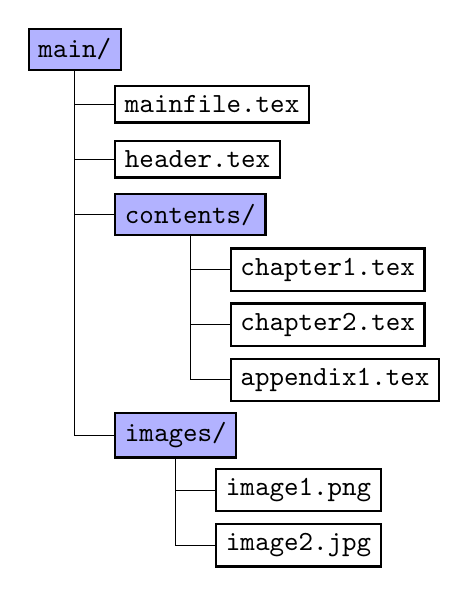
\begin{tikzpicture}[
	every node/.style={draw=black,thick,anchor=west},
	grow via three points={one child at (0.5,-0.7) and two children at (0.5,-0.7) and (0.5,-1.4)},
 	edge from parent path={(\tikzparentnode.south) |- (\tikzchildnode.west)}]
 	\ttfamily
	\node [fill=blue!30] {main/}
		child {node {mainfile.tex}}
		child {node {header.tex}}
%		child {node {defs}}
		child {node [fill=blue!30] {contents/}
			child {node {chapter1.tex}}
			child {node {chapter2.tex}}
			child {node {appendix1.tex}}
		}
		child [missing] {}
		child [missing] {}
		child [missing] {}
		child {node [fill=blue!30] {images/}
			child {node {image1.png}}
			child {node {image2.jpg}}
		}
	;
\end{tikzpicture}
\end{column}
\end{columns}
\end{frame}
\MakeShortVerb|

\begin{frame}[fragile]{\texttt{input} \& \texttt{include}}
\begin{itemize}
\item \verb|\input| and \verb|\include| insert external files at the specified location
\item \TeX\ "jumps" out of the current document, reads elsewhere, and jumps back \pause
\item \TeX\ version: \verb|\input| simply reads the code as if it belonged to the main document
\item \LaTeX\ version: \verb|\include| creates its own \verb|.aux| file (useful when \verb|.aux| is needed)
\item \verb|\includeonly{a.tex,b.tex}| in the preamble allows only the specified files for \verb|\include|
\item \verb|\excludeonly{b.tex,c.tex}| does \emph{not} allow the specified files for \verb|\include| (requires \pkg{excludeonly} package)
\end{itemize}
\end{frame}

\begin{frame}[fragile]{Root Document}
\begin{itemize}
\item After division, only the main document must be compiled
\item[⇒] Constant switching between documents \pause
\item Good editors take care of the work:
\begin{itemize}
\item Definition of main documents possible
\item Automatically compiles the associated main document
\end{itemize}
\end{itemize}
\pause\vfill
\begin{description}
\item[\parbox{2cm}{\vspace{-5.68cm}\flushright\TeX works\\\TeX shop\\\TeX studio}]
Setting \emph{magic comments:}\\\verb*?% !TEX root = ?\meta{Main document}
\begin{lstlisting}
% !TEX root = ../Thesis.tex
% !TEX program = lualatex
% !TEX encoding = utf8
% !TEX spellcheck = en_US
\end{lstlisting}
\item[Overleaf] Menu\,→\,Main Document
\item[Many IDEs] Setting a “project main file”
\end{description}
\end{frame}

\begin{frame}[fragile,t]{Example Main Document}
\begin{lstlisting}
\input{header}

\includeonly{chapter1}
\excludeonly{appendix} % requires excludeonly package!

\begin{document}
\include{chapter1}
\include{chapter2}
...
\appendix
\include{appendix}
\end{document}
\end{lstlisting}
\vfill
⇒ Only \verb|chapter1| is set here, \verb|appendix| is explicitly never included.
\overleaf{tex20}
\end{frame}

\begin{frame}[fragile]{Header Document}{Settings}
\begin{itemize}
\item Page layout
\item Fonts (body text, headings)
\item Formatting of equations
\item …
\item everything before \verb|\begin{document}|
\end{itemize}
\end{frame}

\begin{frame}[fragile,t]{Front Matter}
\begin{itemize}
\item Contains everything up to the first content page
\item Includes author, title, etc.
\item with KOMA: Document option \verb|titlepage=true/false| sets own pages or a title head
\item Environment \verb|\begin{titlepage}| sets a freely designable title page
\item Command \verb|\maketitle| sets predefined front matter
\item Specifications of \verb|\title|, \verb|\author|, \verb|\extratitle| etc. necessary and possible
\end{itemize}
\overleaf{tex14}
\end{frame}

\begin{frame}[fragile,t]{Title Commands in the KOMA Bundle}
\begin{lstlisting}
\documentclass{scrbook}
\begin{document}
\titlehead{\Large University of Smartville}
\subject{Master's Thesis}
\title{Risk Management in the Era of Social Media}
\subtitle{Design of Interactive Apps for Banks and
Insurance Companies}
\author{cand. stup. Ian Imprécis}
\date{February 30, 2024}
\publishers{Supervised by Prof. Dr. Smartypants}
\dedication{For my Mom.}

\maketitle
\end{document}
\end{lstlisting}
\end{frame}

\begin{frame}[fragile,b]{|\textbackslash maketitle| (in the Beamer Class)}
\begin{LTXexample}[pos=b]
\title{Risk Management in the Era of Social Media}
\subtitle{Design of Interactive Apps for Banks and
Insurance Companies}
\author{cand. stup. Ian Imprécis}
\date{30. Februar 2024}

\maketitle
\end{LTXexample}
\end{frame}

\begin{frame}[fragile,t]{Abstract}
\begin{itemize}
\item Environment \verb|abstract| exists for a brief summary of the document
\item Several abstracts possible (e.\,g., English/German etc.)
\end{itemize}
\vfill
\begin{LTXexample}
\begin{abstract}
Here comes a brief summary of the content \dots
\end{abstract}

And here the actual document starts
\dots
\end{LTXexample}
The \texttt{abstract} environment is not available in the \texttt{scrbook}/\texttt{book} class.
\end{frame}

\begin{frame}[fragile]{Lists of Content - TOC, LOF, LOT}
\begin{itemize}
\item Lists compile structured elements
\item Essentially, anything can be included in its own list
\item Common lists:
\begin{itemize}
\item Table of contents \hfill \verb|\tableofcontents|
\item List of figures \hfill \verb|\listoffigures|
\item List of tables \hfill \verb|\listoftables|
\end{itemize}
\item Inclusion of lists in the table of contents: \verb|\setuptoc{toc}{totoc}|
% \item Possible: code list, example list, …
\end{itemize}
\end{frame}

\begin{frame}[fragile]{Footnotes, Marginal Notes}
Additional text that does not fit into the main document/text flow
\begin{itemize}
\item Footnotes \hfill \verb|\footnote{}|
\item Floating margin note \hfill \verb|\marginpar|
\item Margin note (Package \pkg{marginnote}) \hfill \verb|\marginnote|
\end{itemize}
\vfill
Package \pkg{footmisc} offers various options to customize the appearance of footnotes
\end{frame}

\begin{frame}[fragile]{Quotations}
There are dedicated environments for quotations:
\begin{itemize}
\item \verb|quote| for short quotations
\item \verb|quotation| for longer quotations
\item \verb|verse| for poems
\end{itemize}
Package \pkg{csquotes} adjusts finer points of quotation marks for non-English text.
\vfill
\begin{lstlisting}
\begin{quote}
alea iacta est \hfill\textit{Caesar}
\end{quote}
\end{lstlisting}
\end{frame}

\begin{frame}[fragile]{References}
\begin{itemize}
\item Elements can be labeled with \verb|\label{}|
\item Possible elements are headings (sections etc.), \verb|table|, \verb|figure|, formulas, …
\item Referencing with \verb|\ref{}| or \verb|\cref| (Package \pkg{cleveref})
\end{itemize}
\end{frame}

\begin{frame}[fragile,t]{Links in the Document}{hyperref}
\begin{itemize}
\item Package \pkg{hyperref} makes references clickable in the PDF
\item \verb|\ref| and \verb|\cite| are automatically linked
\item URLs can be specified with \verb|\url{}|
\item Named links with \verb|\href{}{}|
\end{itemize}
\uncover<2>{To avoid problems, load \pkg{hyperref} as the last package!}
\vfill
\begin{LTXexample}
\url{http://xkcd.com}\\
\href{mailto:mail@latexkurs.de}{\huge\Letter}
\end{LTXexample}
\end{frame}

\begin{frame}[fragile]{Front Matter}
\begin{itemize}
\item Command |\frontmatter| switches to Roman page numbers
\item |\mainmatter| to normal numbering
\item |\backmatter| to appendix \\ in other document classes: only |\appendix|
\item Numbering starts anew\\(dependent on document class A, B, C, …)
\item Sections in the appendix as usual with |\chapter|, |\section|, etc.
\end{itemize}
\vfill
\begin{lstlisting}
\frontmatter
\mainmatter
\backmatter
\end{lstlisting}
\end{frame}

\begin{frame}{Application}
\begin{arbeitsauftrag}
Add the following elements to your document:
\begin{itemize}
\item Title page
\item Table of contents
\item List of figures
\item List of tables
\item Appendix
\end{itemize}
\end{arbeitsauftrag}
\end{frame}


%%%%%%%%%%%%%%%%%%%%%%%%%%%%%%%%%%%%%%%%%%%%%%%%%%%%%%%%%%%%%%%%%%%%%%%%%%%%%%%%%%%%%%%%%%%%%%%%%%%%%%%%%%
\teil{Diagrams}
%%%%%%%%%%%%%%%%%%%%%%%%%%%%%%%%%%%%%%%%%%%%%%%%%%%%%%%%%%%%%%%%%%%%%%%%%%%%%%%%%%%%%%%%%%%%%%%%%%%%%%%%%%

\begin{frame}{Diagrams}
\begin{itemize}
\item A diagram is a graphical representation of data, facts, or information.
\item Information should be the primary focus.
\item Diagrams should fit into the document:
\begin{itemize}
\item appropriate dimensions
\item labeling in the same font style
\end{itemize}
\end{itemize}

Recommendation for diagrams in \LaTeX: \pkg{pgfplots}
\end{frame}

\begin{frame}[fragile]{pgfplots}
Configuration using \verb|\pgfplotsset{|\meta{options}|}|. The package author recommends specifying the current version for future compatibility.
\begin{lstlisting}
\usepackage{pgfplots}
\pgfplotsset{compat=1.18}
\end{lstlisting}
\pause
\pkg{pgfplots} is based on \href{http://ctan.org/pkg/pgf}{\TikZ/PGF} and therefore is within a |tikzpicture| environment:
\begingroup
\pgfplotsset{scale=0.5}
\begin{LTXexample}[pos=r, explpreset={}, preset=, rframe={}]
\begin{tikzpicture}
  \begin{axis}
    ...
  \end{axis}
\end{tikzpicture}
\end{LTXexample}
\endgroup
\overleaf{tex15}
\end{frame}


\begin{frame}{Types of Axes}
Various types of axes available: \\[1em]
\texttt{\textbackslash begin\{}\meta{axis type}\verb|\}[|\meta{options}\verb|]|\\
\quad\meta{content}\\
\texttt{\textbackslash end\{}\meta{axis type}\verb|\}|

\vfill

\begin{tabular}{rl}
\verb|axis| & linear coordinate axes\\
\verb|semilogyaxis| & linear $x$-axis, logarithmic $y$-axis\\
\verb|semilogxaxis| & logarithmic $x$-axis, linear $y$-axis\\
\verb|loglogaxis| & both axes logarithmic\\
\verb|polaraxis| & polar coordinates\footnote{with \verb|\textbackslash usepgfplotslibrary\{polar\}|}\\
\verb|smithchart| & Smith chart\footnote{with \verb|\textbackslash usepgfplotslibrary\{smithchart\}|}\\
\verb|ternaryaxis| & ternary diagram\footnote{with \verb|\textbackslash usepgfplotslibrary\{ternary\}|}
\end{tabular}
\end{frame}


\begin{frame}[fragile,t]{Adding Data}%\verb|\textbackslash addplot|}
\verb|\addplot [|\meta{options}\verb|] {|\meta{input data}\verb|};|\\%\meta{additional TikZ commands}|;|\\
\verb|\addplot+[|\meta{options}\verb|] {|\meta{input data}\verb|};|%\meta{additional TikZ commands}|;|
\pdfmarginpar{While the specified options at \texttt{addplot} override the global/standard options, \texttt{addplot+} only adds the specified options to the global ones.}\vfill
\begin{LTXexample}[pos=r, explpreset={}, preset=\small, rframe={}]
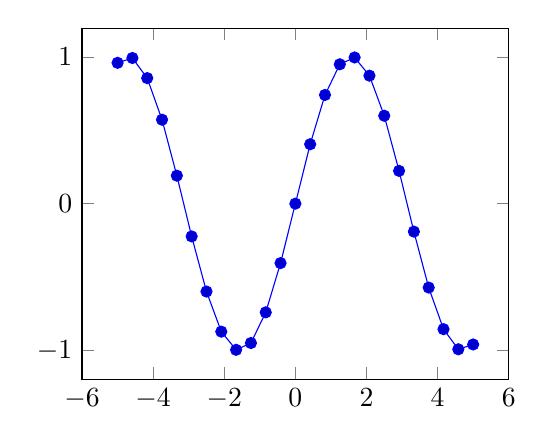
\begin{tikzpicture}
  \begin{axis}
    \addplot{sin deg(x)};
  \end{axis}
\end{tikzpicture}
\end{LTXexample}
\end{frame}

\begin{frame}[fragile,t]{Coordinate Input}
\verb|\addplot [|\meta{options}\verb|] coordinates {|\meta{coordinates}\verb|};|\vfill
\begin{LTXexample}[pos=r, explpreset={}, preset=\small, rframe={}]
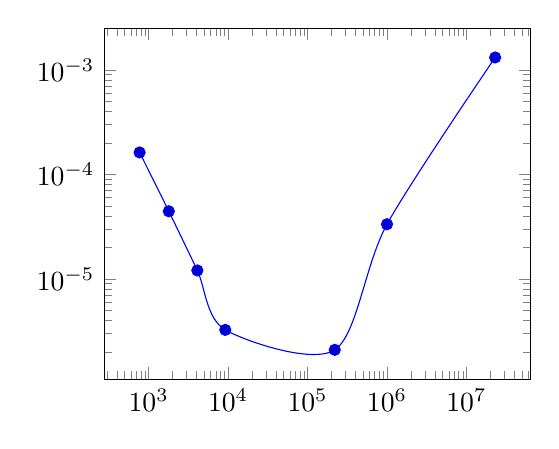
\begin{tikzpicture}
  \begin{loglogaxis}
    \addplot+[smooth]
     coordinates {
      (769, 1.6227e-04)
      (1793, 4.4425e-05)
      (4097, 1.2071e-05)
      (9217, 3.2610e-06)
      (2.2e5, 2.1E-6)
      (1e6, 0.00003341)
      (2.3e7, 0.00131415)
    };
  \end{loglogaxis}
\end{tikzpicture}
\end{LTXexample}
\end{frame}


\begin{frame}[fragile,t]{Data Tables}
\verb|\addplot [|\meta{options}\verb|] table [|\meta{column selection}\verb|] {|\meta{table}\verb|};|\vfill
\begin{LTXexample}[pos=r, explpreset={}, preset=\small, rframe={}]
\begin{tikzpicture}
  \begin{axis}
    \addplot table [
      only marks,
    ] {
      x    y    myvalue 
      0.5  0.2  0.25
      0.2  0.1  1.5
      0.7  0.6  0.75
      0.35 0.4  0.125
      0.65 0.1  2
    };
  \end{axis}
\end{tikzpicture}
\end{LTXexample}
\end{frame}


\begin{frame}[fragile,t]{Data in External Files}
\verb|\addplot [|\meta{options}\verb|] table [|\meta{column selection}\verb|] {|\meta{file path}\verb|};|\vfill
\begin{LTXexample}[pos=r, explpreset={}, preset=\small, rframe={}]
\begin{tikzpicture}
  \begin{axis}
    \addplot [no markers]
      table
      [x=time, y=values]
      {data.dat};
  \end{axis}
\end{tikzpicture}
\end{LTXexample}
\pause
Package \pkg{pgfplotstable} allows post-processing of existing tables (e.g., inserting a trendline).
\end{frame}

\begin{frame}[fragile]{Labels}
\begin{tabular}{rll}
Key & Values & Function\\\midrule
\verb|title| & Text & Title above the diagram\\
\verb|x|/\verb|ylabel| & any text & Label of the $x$- or $y$-axis  \\
\verb|x|/\verb|ymin|/\verb|max| & value & limits axis to range\\
\verb|mark| & \verb|*|, \verb|x|, \verb|+|, \verb|o|, … & customize coordinate markers\\
\verb|x|/\verb|ytick| & list & explicitly specify coordinate ticks\\
\verb|minor tick num| & number & number of minor ticks\\
\verb|grid| & \verb|major|, \verb|minor| & display gridlines in the background
\end{tabular}
\end{frame}

\begin{frame}[fragile,t]{Legends}
\verb|\addlegendentry{|\meta{description}\verb|}|\vfill
\begin{LTXexample}[pos=r, explpreset={}, preset=\small, rframe={}]
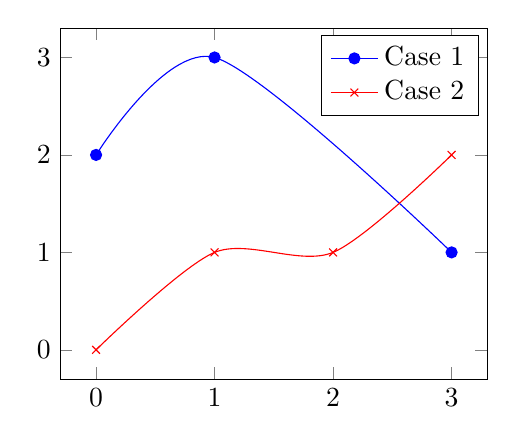
\begin{tikzpicture}
\begin{axis}
  \addplot[smooth,mark=*,blue] coordinates {
    (0,2) (1,3) (3,1)
  };
  \addlegendentry{Case 1}
  \addplot[smooth,color=red,mark=x] coordinates {
    (0,0) (1,1) (2,1) (3,2)
  };
  \addlegendentry{Case 2}
\end{axis}
\end{tikzpicture}
\end{LTXexample}
\end{frame}

\begin{frame}[fragile,t]{Axis Placement}
\verb|axis y line=|\meta{placement}, \verb|axis x line=|\meta{placement}\vfill
\begin{LTXexample}[pos=r, explpreset={}, preset=\small, rframe={}]
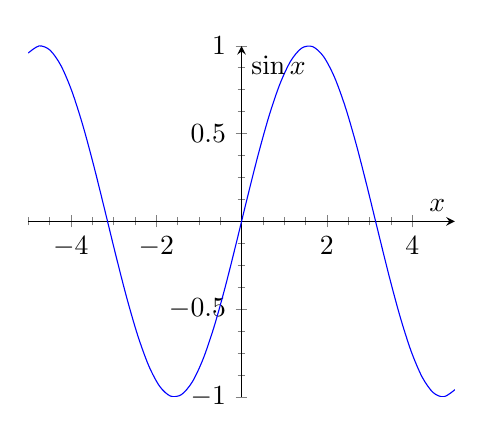
\begin{tikzpicture}
\begin{axis}[
minor tick num=3,
axis y line=center,
axis x line=middle,
xlabel=$x$,ylabel=$\sin x$
]
\addplot[smooth,blue,mark=none,
domain=-5:5,samples=40]
{sin(deg(x))};
\end{axis}
\end{tikzpicture}
\end{LTXexample}
\end{frame}

\begin{frame}[fragile,t]{Error Bars}
Errors can be set using the options \verb|error bars/|\meta{key}\verb|=|\meta{value}.\vfill
\begin{LTXexample}[pos=r, explpreset={}, preset=\small, rframe={}]
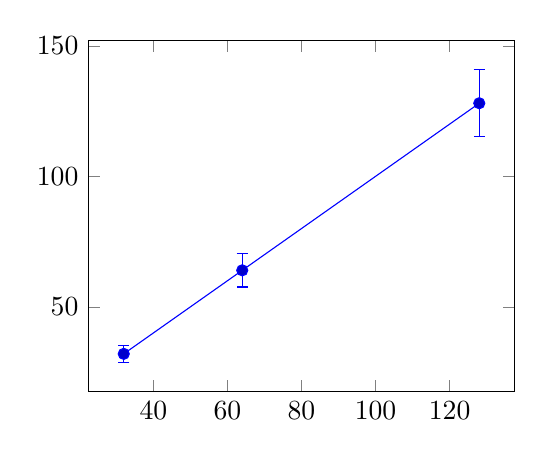
\begin{tikzpicture}
\begin{axis}
  \addplot+[
   error bars/y dir=both,
   error bars/y fixed relative=.1,
  ] table [x=x,y=y]
  {x    y
   32     32
   64     64
   128    128
  };
\end{axis}
\end{tikzpicture}
\end{LTXexample}
\end{frame}

\begin{frame}[fragile,t]{Error Bars}
Individual errors can be specified with \verb|+-| (symmetric) or \verb|+=| and \verb|-=| (asymmetric):\vfill
\begin{LTXexample}[pos=r, explpreset={}, preset=\small, rframe={}]
\begin{tikzpicture}
\begin{axis}
  \addplot+[
    error bars/.cd,
    x dir=both,
    x explicit,
    y dir=both, 
    y explicit,
  ] coordinates {
    (1,1) += (0.4,0.2) 
          -= (0.1,0.1)
    (3,2) -= (1,0)
    (4,5) +- (0.3,0.2)
  };
\end{axis}
\end{tikzpicture}
\end{LTXexample}
\end{frame}

\begin{frame}[fragile,t]{Error Bars}
Errors can also come from a table:\vfill
\begin{LTXexample}[pos=r, explpreset={}, preset=\small, rframe={}]
\begin{tikzpicture}
  \begin{axis}
    \addplot [only marks, mark=x, 
    error bars/.cd,
    y dir=both, y explicit,]
      table
      [x=time, y=values, y error=error]
      {data.dat};
  \end{axis}
\end{tikzpicture}
\end{LTXexample}
\end{frame}


\begin{frame}[fragile,t]{Histograms}
Histograms with option \verb|hist={|\meta{histogram options}\verb|}|\vfill
\begin{LTXexample}[pos=r, explpreset={}, preset=\small, rframe={}]
\begin{tikzpicture}
  \begin{axis}
    \addplot+[
      fill=blue!40!white,
      mark={},
      hist={
        data=y, 
        bins=10
      }
    ] table {data.dat};
  \end{axis}
\end{tikzpicture}
\end{LTXexample}
Interesting options:\\\verb|cumulative| for cumulative histogram\\\verb|density| normalized to 1
\end{frame}


\begin{frame}[fragile,t]{Bar Charts}
Option \verb|xbar| creates horizontal bar chart, \verb|ybar| creates vertical bar chart\vfill
\begin{LTXexample}[pos=r, explpreset={}, preset=\small, rframe={}]
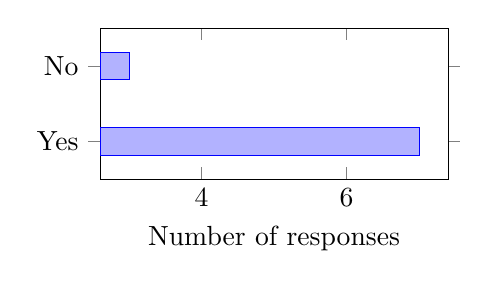
\begin{tikzpicture}
\begin{axis}[
 xbar,
 width=6cm, height=3.5cm,
 enlarge y limits=0.5,
 xlabel={Number of responses},
 symbolic y coords={Yes,No},
 ytick=data,
]
 \addplot coordinates
  {(3,No) (7,Yes)};
\end{axis}
\end{tikzpicture}
\end{LTXexample}
\end{frame}


\begin{frame}[fragile,t]{Bar Charts}
Option \verb|xbar| creates horizontal bar chart, \verb|ybar| creates vertical bar chart\vfill
\begin{LTXexample}[pos=r, explpreset={}, preset=\small, rframe={}]
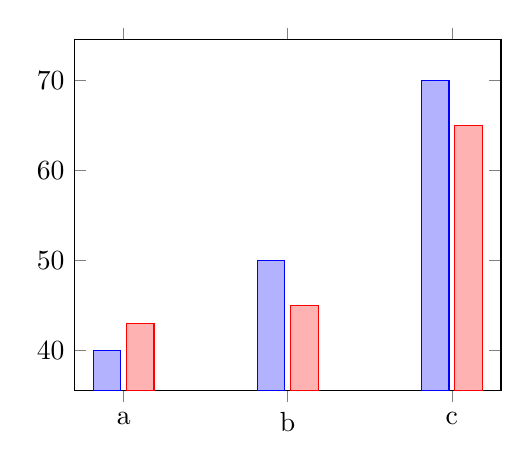
\begin{tikzpicture}
\begin{axis}[
 ybar,enlargelimits=0.15,
 symbolic x coords={a,b,c},xtick={a,b,c},
]
 \addplot coordinates 
 {(a,40) (b,50) (c,70)};
 \addplot coordinates 
 {(a,43) (b,45) (c,65)};
 \

addplot coordinates 
 {(a,13) (b,25) (c,35)};
\end{axis}
\end{tikzpicture}
\end{LTXexample}
\end{frame}



\begin{frame}[fragile,t]{Boxplots}
\verb|\usepgfplotslibrary{statistics}| allows generation of boxplots:\vfill
\usepgfplotslibrary{statistics}
\begin{LTXexample}[pos=r, explpreset={}, preset=\small, rframe={}]
\begin{tikzpicture}
  \begin{axis}
    \addplot+[
    boxplot prepared={
      median=4000,
      upper quartile=5500,
      lower quartile=3000,
      upper whisker=1200,
      lower whisker=15000,
    } ] coordinates {};
  \end{axis}
\end{tikzpicture}
\end{LTXexample}
\end{frame}

\begin{frame}[fragile,t]{3D Plots}% \verb|\textbackslash addplot3|}
\verb|\addplot3 [|\meta{options}\verb|] {|\meta{input data}\verb|};| \vfill
\begin{LTXexample}[pos=r, explpreset={}, preset=\small, rframe={}]
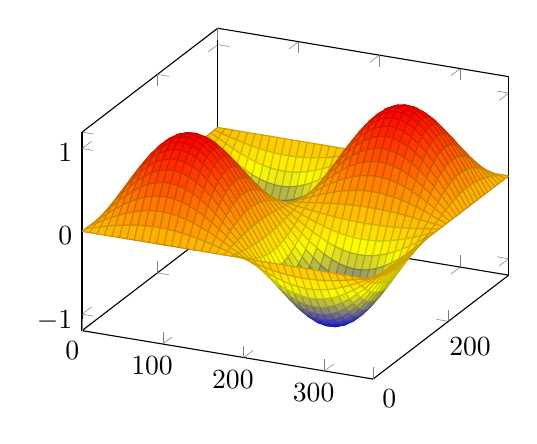
\begin{tikzpicture}
  \begin{axis}
    \addplot3[
      surf,
      domain=0:360,
      samples=40,
    ]
    {sin(x)*sin(y)};
  \end{axis}
\end{tikzpicture}
\end{LTXexample}
\end{frame}

%% Export TikZ diagrams from R: R package “TikZDevice”

\nocite{mathmode, amsmath, tabularray, booktabs, dante:wissarbeit, koma-en, pgfplots}
\begin{frame}[allowframebreaks]{Further Reading}
\printbibliography
\end{frame}


\begin{frame}<handout:1>{Teaching Evaluation}

\begin{columns}
	\column{.4\textwidth}
	\href{https://evasys.uni-mannheim.de/evasys/online.php?p=\kursAB{\evallosungA}{\evallosungB}}{\qrcode[height=\textwidth]{https://evasys.uni-mannheim.de/evasys/online.php?p=\kursAB{\evallosungA}{\evallosungB}}}
	\column{.55\textwidth}
	\begin{tabbing}
	\textbf{Losung:\quad}\=\url{evasys.uni-mannheim.de} \kill
	\textbf{Link:} \> \href{https://evasys.uni-mannheim.de/evasys/online.php?p=\kursAB{\evallosungA}{\evallosungB}}{\texttt{evasys.uni-mannheim.de}} \\
	\textbf{TAN:} \> \href{https://evasys.uni-mannheim.de/evasys/online.php?p=\kursAB{\evallosungA}{\evallosungB}}{\texttt{\kursAB{\evallosungA}{\evallosungB}}}
	\end{tabbing}
\end{columns}
\end{frame}


\AtEndDocument{\frame{\centering \Huge Happy \TeX ing}}

\end{document}